\documentclass{beamer}

\usepackage{beamer_tom}
\graphicspath{{./images/}}

\institute{INRIA - Parietal}
\author{T. Moreau}
\title{
    Extraction of Nystagmus Patterns from {Eye-Tracker} Data\\
    with Convolutional Sparse Coding
}

\collaborators{
    C. Lalanne$^1$, M. Rateaux$^{1,2}$,
    L. Oudre$^{1,3}$, M. Robert$^{1, 2}$\\[.5em]
    {
        $^1$CNRS - Centre  Borelli, $^2$APHP - Hôpital Necker,
        $^3$Université Paris 13 - L2TI
    }
    \vskip-2em
}
\setbeamertemplate{title page}[frame]
\def\extraLogo{\includeLogos[.7em]{logo_cnrs,logo-parisdescartes,
                                  logo_UP13,logo_UPSA}}



\newcommand{\highlightbox}[1]{
    \begin{beamercolorbox}[rounded=true,
                           shadow=true]{title}
        #1
    \end{beamercolorbox}}

\begin{document}

    \begin{frame}
        \titlepage
    %	\biblio{}
    \end{frame}

    \frame{
        \frametitle{Pathological Infantile Nystagmus}

        \begin{columns}[c]
            \column{.5\textwidth}
            \begin{itemize}
                \item Sporadic movement of the eye.
                \item Link to several conditions:\\Gliomas, albinism, down syndrom, ...
                \item Classification of 16 different Waveforms [Dell'Osso et al. 75]
            \end{itemize}
            \column{.5\textwidth}
            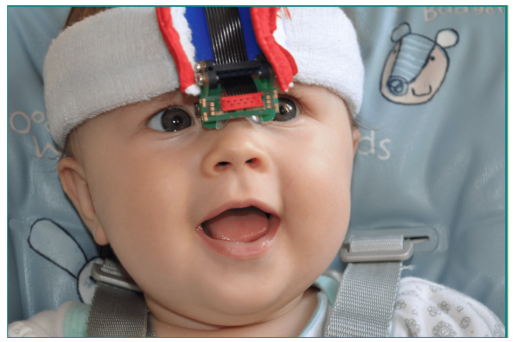
\includegraphics[width=\textwidth]{eyefant.png}
            \keypoint{Recording the nystagmus with an eye tracker}
        \end{columns}

        \vskip2em
        Can extract the waveform automatically?
        \strongpoint{Use Convolutional Dictionary Learning!}
    }

    \frame[t]{
        \frametitle{Local structure in signals}

        \visible<5->{
            \textbf{Key idea}: decouple the localization of the
                                patterns and their shape}
        \vskip.5em%
        \centering%
        \only<1>{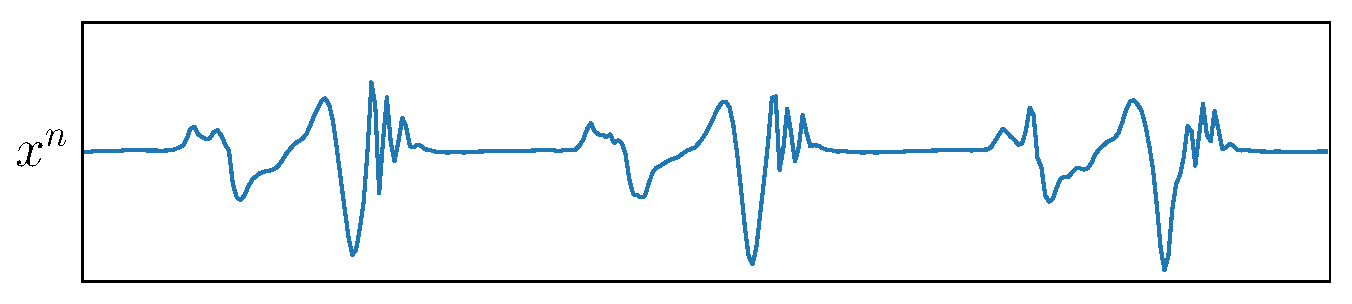
\includegraphics[width=\textwidth]{intro_csc_0}}%
        \only<2>{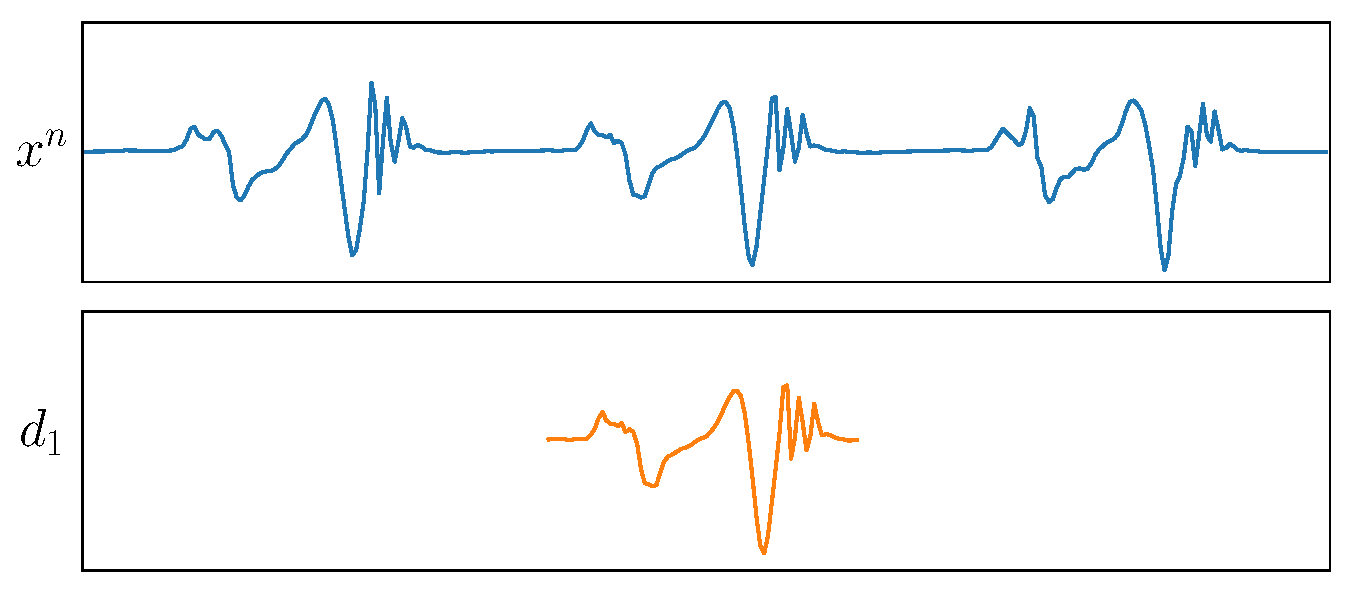
\includegraphics[width=\textwidth]{intro_csc_1}}%
        \only<3>{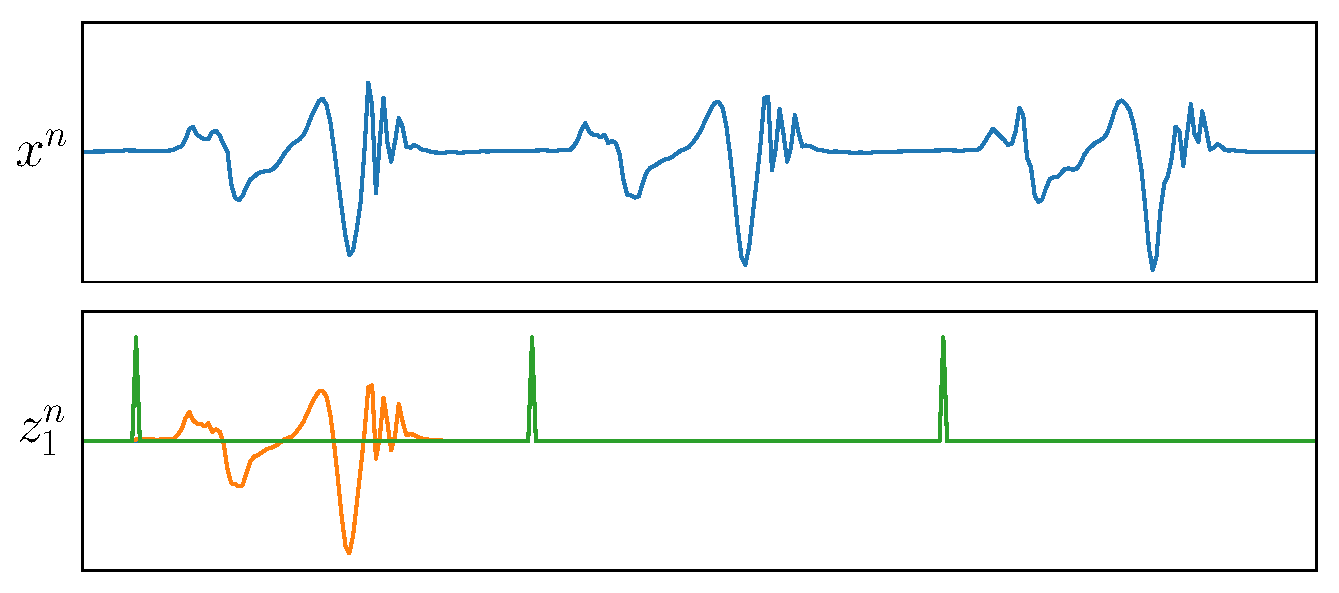
\includegraphics[width=\textwidth]{intro_csc_2}}%
        \only<4>{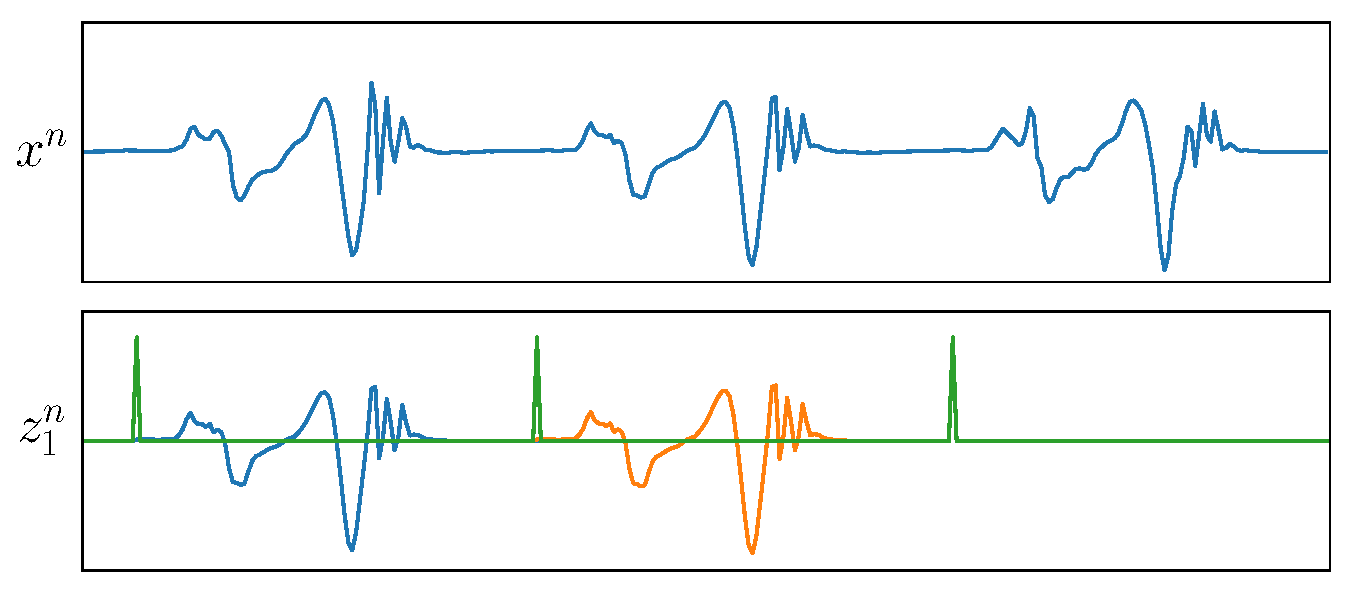
\includegraphics[width=\textwidth]{intro_csc_3}}%
        \only<5>{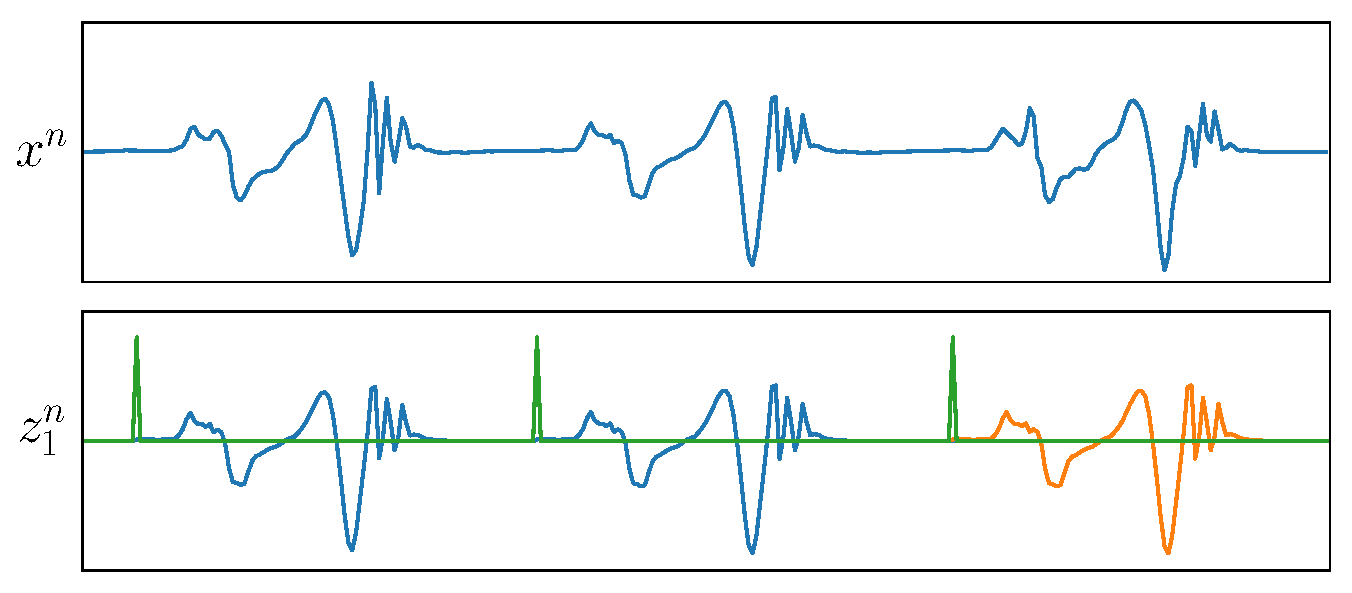
\includegraphics[width=\textwidth]{intro_csc_4}}%
        \only<6->{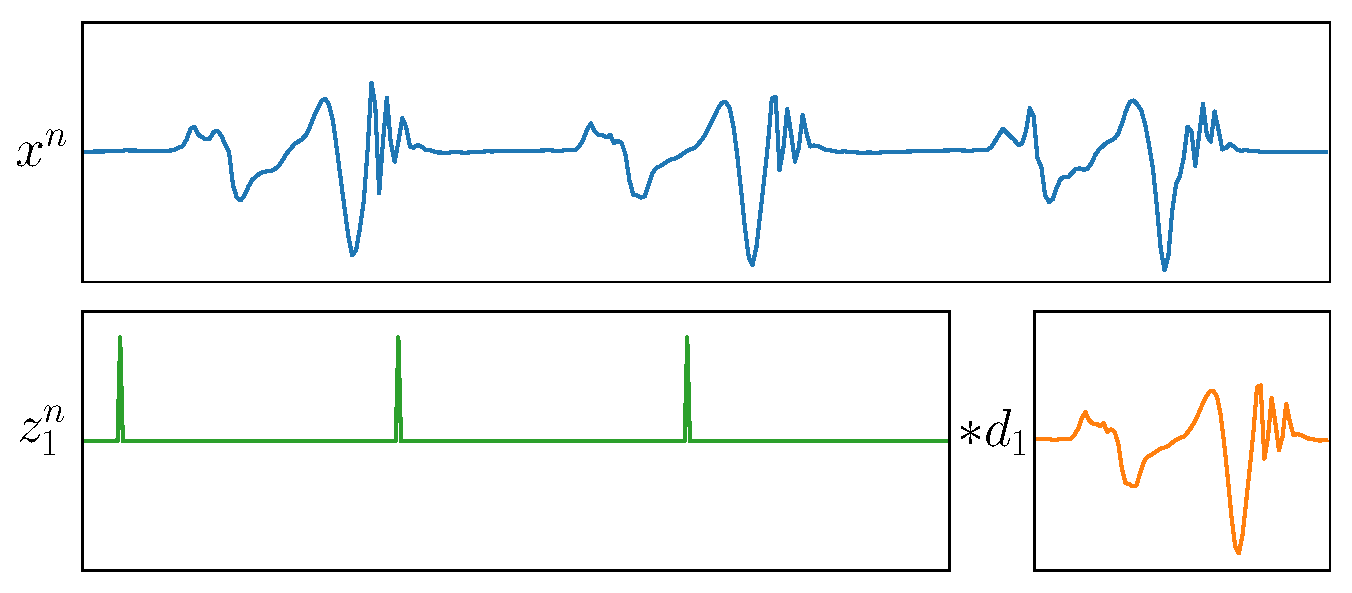
\includegraphics[width=\textwidth]{intro_csc_5}}%
        \vskip0em%
        \only<7>{%
            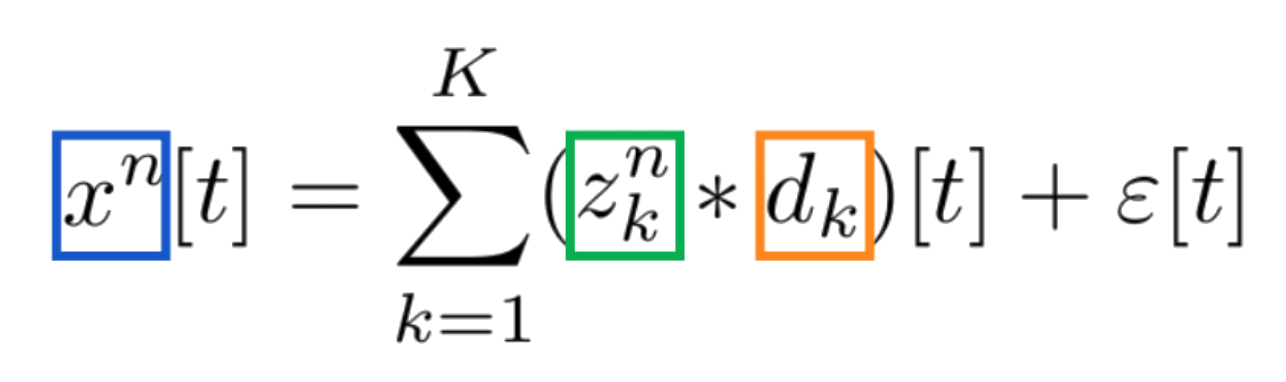
\includegraphics[width=.6\textwidth]{csc_explain_eq_color}%
        }
    }
    \frame[c]{
        \frametitle{CSC as an optimization problem}

        Estimation is done with the following optimization problem\\[1em]
        {
            \centering
            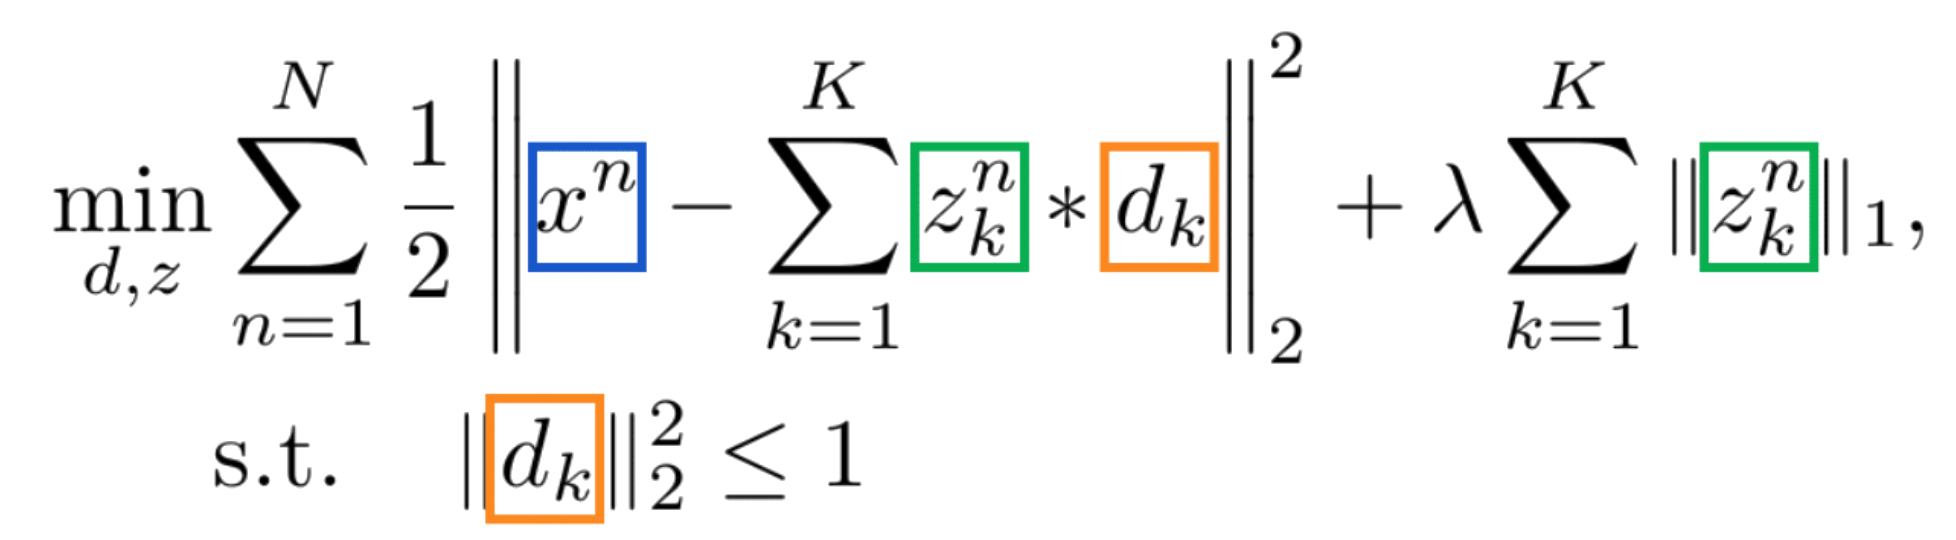
\includegraphics[width=.7\textwidth]{csc_eq_l1.png}\\[2em]
        }

        \begin{columns}[c]
            \column{.4\textwidth}
            Non-convex problem but bi-convex.

            \column{.6\textwidth}
            Solved with alternate minimization:
            \begin{itemize}
                \item Fix $D$ and minimize on $z$
                \item Fix $z$ and minimize on $D$
            \end{itemize}

        \end{columns}
        \vskip2em
        {\hskip8em $\Rightarrow$ Local minima $z, D$\\}
    }

    \frame[t]{
        \frametitle{Eyetracker recording}
        \vskip2em
        {\centering\alt<2->{
            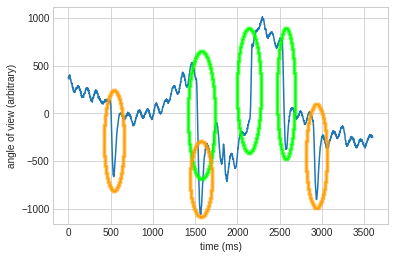
\includegraphics[width=.7\textwidth]{angle_of_view_highlighted}\\[.5em]
            \begin{itemize}
                \item Eye blinks artifacts
                \item Super imposed gaze movement: low freq + saccades.
            \end{itemize}
        }{
            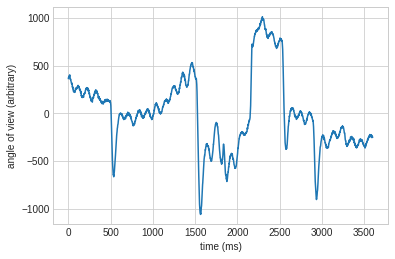
\includegraphics[width=.7\textwidth]{angle_of_view}\\[.5em]
        }}
    }

    \frame{
        \frametitle{Joint detrending and CDL}

        Ad hoc detrending tends to alter the waveform
        \begin{itemize}
            \item Filtering \keypoint{break harmonics}
            \item TV-L1 \keypoint{hard to chose the reg. parameter}
        \end{itemize}

        \vskip2em
        Idea, joint detrending with CDL:
        \[
            \argmin_{z, D, y} \frac12\|x - z*D - y\|_2^2
                + \lambda \|z\|_1 + \lambda_{TV}\|\nabla y\|_1
        \]
        \begin{itemize}
            \item Does not complexify the optimization (bi-convex)
            \item Equivalent to iterative application of a detrending method
            \item Both components will be co-adapted
        \end{itemize}

    }

    \frame{

        \frametitle{Pattern recovery on simulated data}
        We evaluate the pattern recovery of our method on simulated data.
        {\centering
        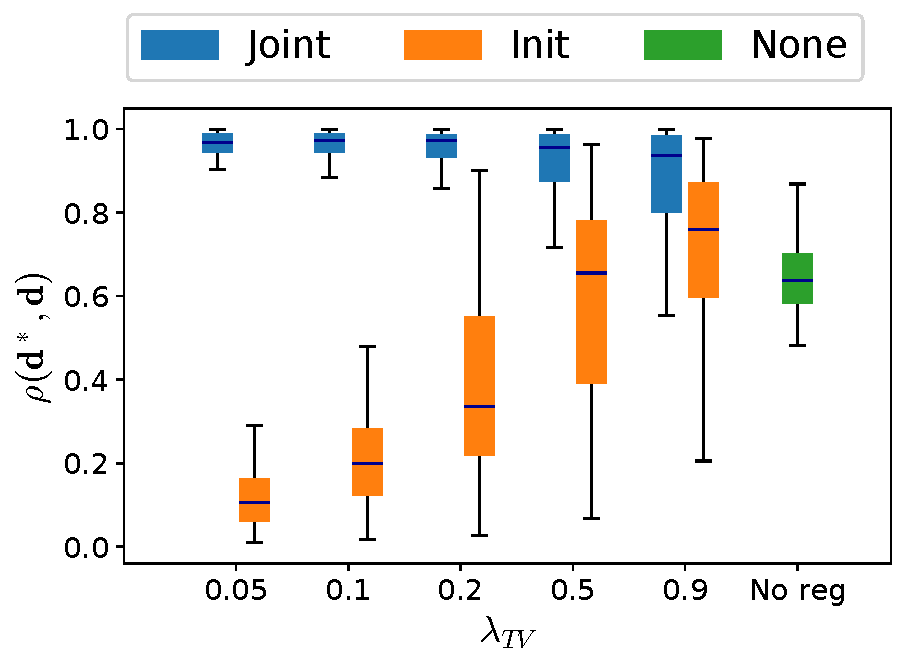
\includegraphics[width=.7\textwidth]{pearson_reg=0,5.pdf}\\}
    }

    \frame{
        \frametitle{Qualitative results on real signals}

        Learn nystagmus waveform on real signals\\[.5em]
        {\centering
        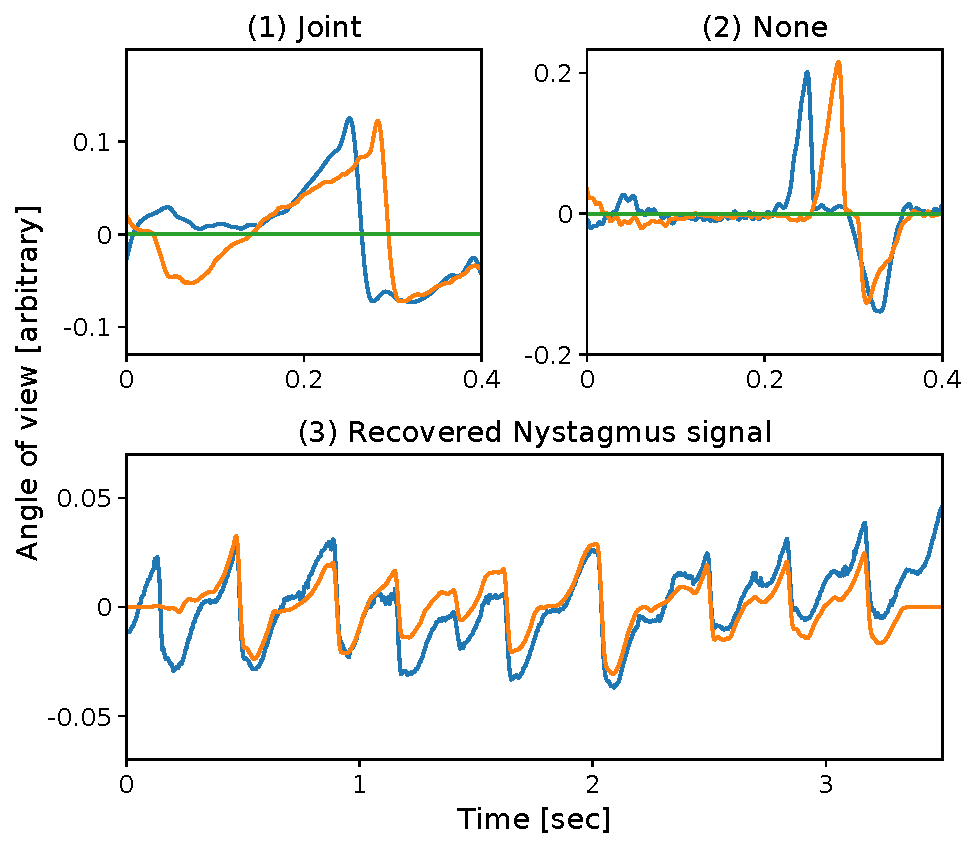
\includegraphics[width=.7\textwidth]{pattern_trend_2.pdf}\\
        }

    }

    {\usebackgroundtemplate{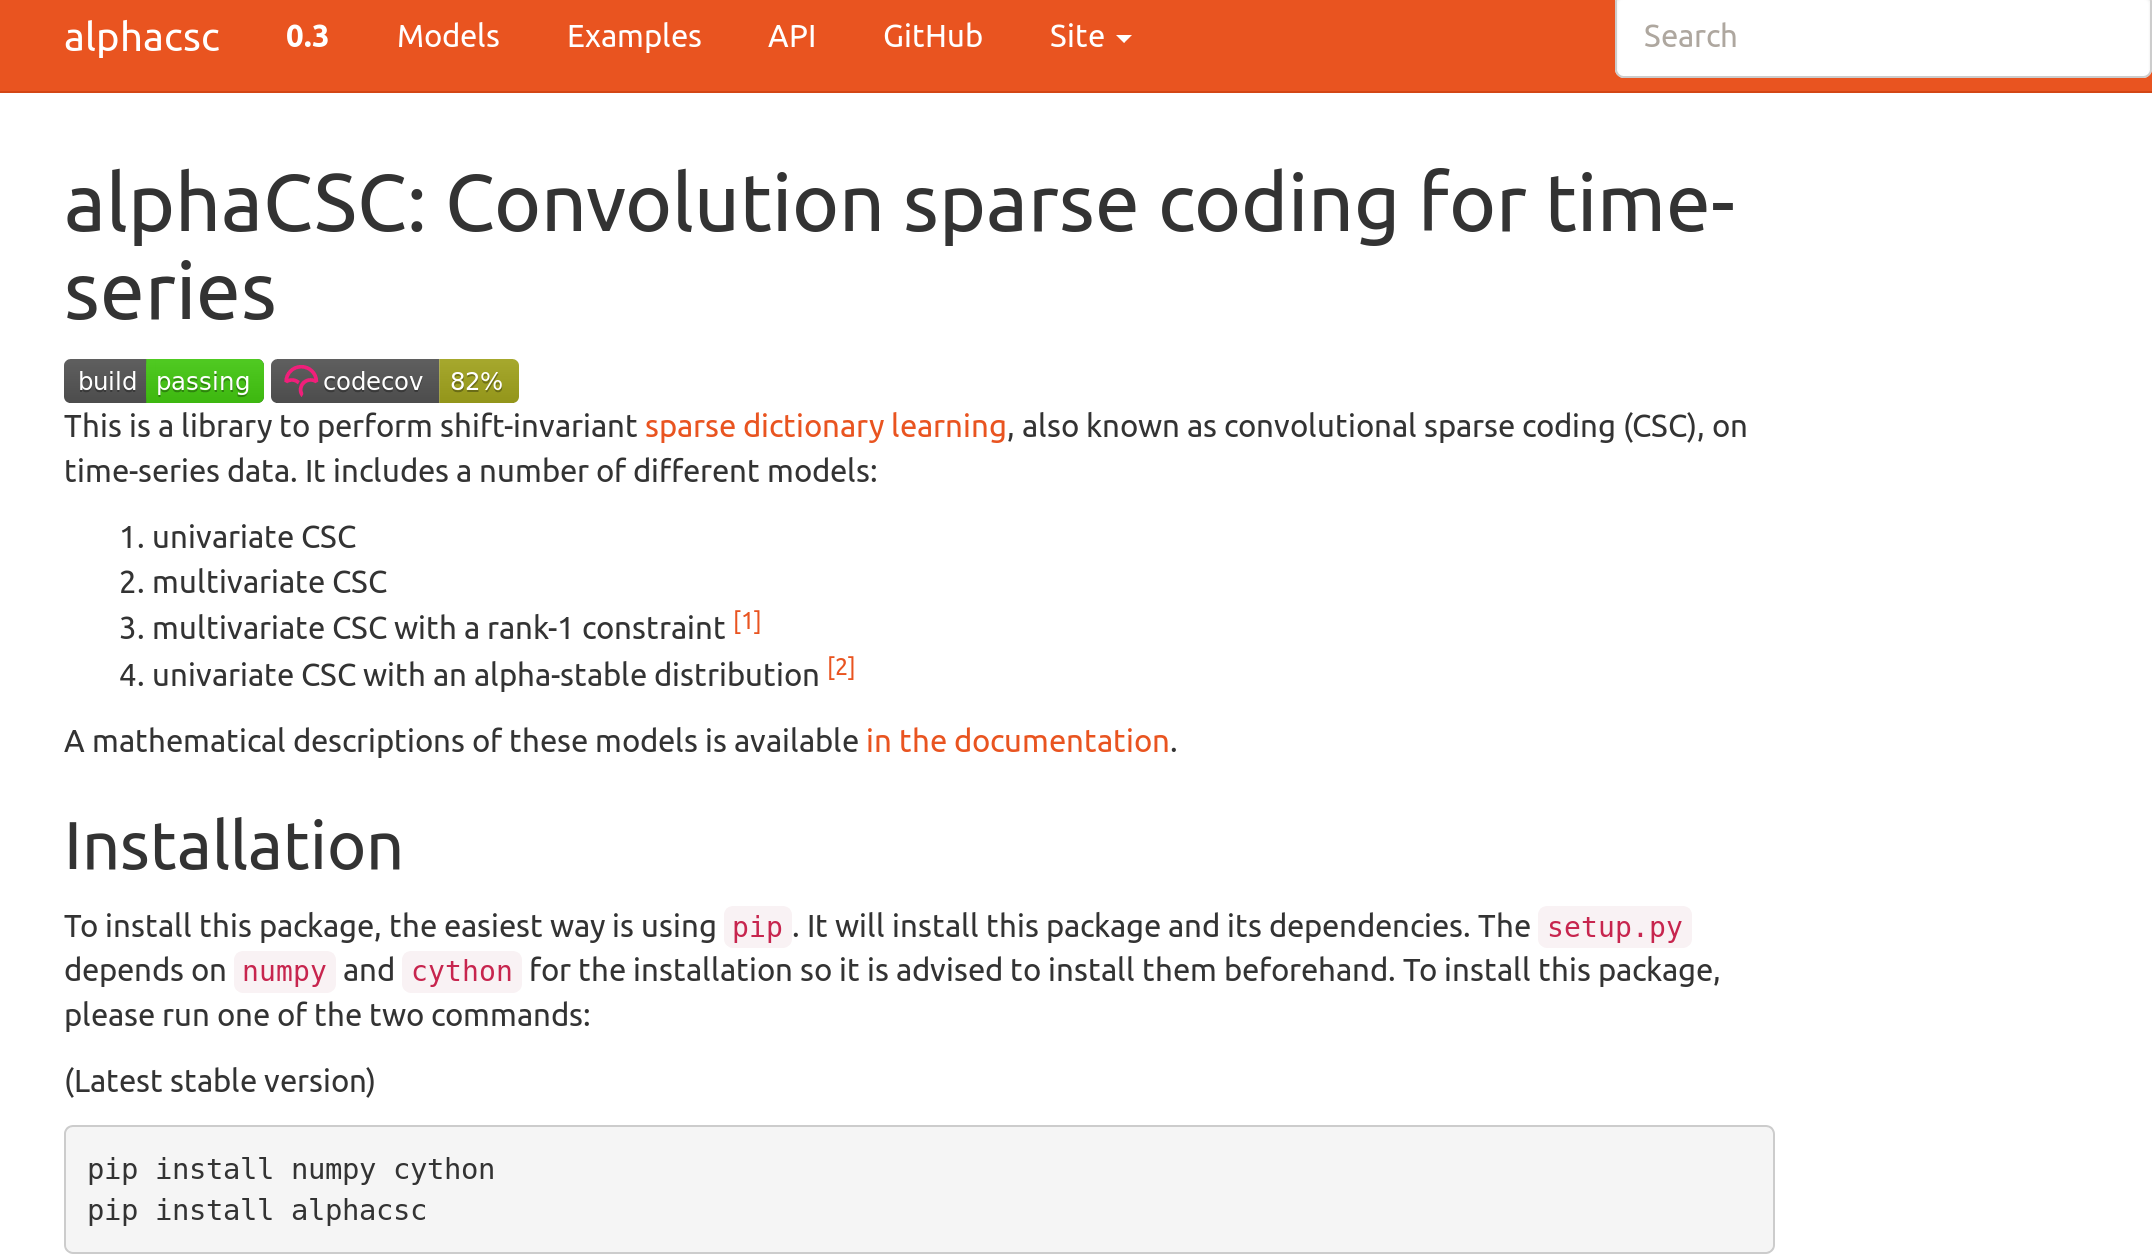
\includegraphics[width=\paperwidth]{alphacsc}}%
    \frame{
        \begin{columns}
            \column{.5\textwidth}
            \column{.4\textwidth}
            \highlightbox{Python code online:\\
                            https://alphacsc.github.io\\[1em]
                            \texttt{pip install alphacsc}}
            \vskip2em
                \highlightbox{Examples reproduce figures from this talk!}

        \end{columns}
    }}

    \frame{
        \frametitle{Extraction of Nystagmus Patterns from {Eye-Tracker} Data\\
                    with Convolutional Sparse Coding}

        {
            \centering\Large\bf
            Thanks for your attention!\\[3em]
        }


        
\includegraphics[height=.8em]{github}~\textbf{alphacsc} :  alphacsc.github.io\\[1em]

        Slides are on my web page:\\[1em]
        \hskip5em\includegraphics[height=.8em]{website} tommoral.github.io
        \hskip4em 
\includegraphics[height=.8em]{twitter} @tomamoral
    }




\end{document}
